\documentclass[a4paper, 11pt]{article}
\usepackage[ngerman]{babel}
%ä und so
\usepackage[utf8]{inputenc}
\usepackage[T1]{fontenc}
\usepackage{amsmath}
\usepackage{amsthm}
\usepackage{amsbsy}

\usepackage{mathrsfs}
\usepackage{amssymb}
\usepackage{amstext}
\usepackage{amsfonts}
\usepackage{float}
\usepackage{graphicx}
\usepackage{esdiff}
\usepackage{hyperref}
\usepackage{geometry}
\geometry{top = 20mm, bottom = 20 mm, left = 25mm, right = 25mm}


\usepackage{setspace}
\onehalfspacing

\usepackage{fancyhdr}
\usepackage{wrapfig}
%\usepackage[hyphens]{url}
%\urlstyle{sf}
%\usepackage[hidelinks]{hyperref}
%\usepackage{breakurl}
%\hypersetup{colorlinks=false}
\usepackage{multirow}
\usepackage[bottom]{footmisc}

%\usepackage{svg}

\title{Mechanik - Messung der Erdbeschleunigung mit dem Pendel und Schwingungen von gekoppelten Pendeln}
\author{Gruppe 2 \\ \\ Adelind Elshani \\ Olexiy Fedorets}
\date{\today}

% !TeX spellcheck = de_DE
\begin{document}


\begin{titlepage}
	\vspace*{\fill}
	\begin{center}
		\vskip -0.25\textheight
		\vfill
		\newcommand{\Line}{\rule{\linewidth}{0.6mm}}
		\Line 
		{\let\newpage\relax\maketitle}
		\Line 
		\vfill
	\end{center}
	\vspace*{\fill}
	\thispagestyle{empty}
\end{titlepage}





\newpage
\thispagestyle{empty}
\tableofcontents
\newpage

%Kopf- und Fußzeile
\pagestyle{fancy}
\fancyhf{}
%Kopfzeile links bzw. innen
\fancyhead[L]{\nouppercase{\leftmark}}
%Kopfzeile rechts bzw. außen
\fancyhead[R]{\thepage}
%Linie oben
\renewcommand{\headrulewidth}{0.5pt}
\fancyfoot[C]{\thepage}


\setcounter{page}{1}

\section{Einleitung}
Zu der Versuchsreihe Mechanik werden zwei Experimente durchgeführt. Das erste Experiment beschäftigt sich mit der Messung der Erdbeschleunigung anhand eines Pendels. Mit dem zweiten Versuch werden die Schwingungen von gekoppelten Pendeln analysiert.  


\section{Messung der Erdbeschleunigung}

\subsection{Grundlagen} 

Das einfache mathematische Pendel ist die idealisierte Form eines Pendels. Es besteht aus einer schweren Masse, dass man annähernd als punktförmig betrachten kann und an einem masselosen Faden aufgehängt ist. Die Schwerkraft $F_g = m_s \cdot g$ bewirkt, dass das Pendel in der Ruhelage senkrecht hängt. Wird das Pendel  nun um einen genügend kleinen Winkel $\phi_{max}$ aus der Ruhelage ausgelenkt, so entsteht ein rückstellendes Drehmoment $l\cdot F_r$. Dies bewirkt eine harmonische Schwingung aufgrund des Trägheitsmomentes des Pendels. Daraus ergibt sich die Bewegungsgleichung
\begin{equation} 
J \cdot \ddot \phi = -m_s \cdot g \cdot l \cdot \cos(\phi)\approx -m_s \cdot g \cdot l \cdot \phi,
\end{equation}
dabei beschreibt $J = m_t \cdot l^2$ das Trägheitsmoment des Pendelkörpers mit der Entfernung $l$ vom Aufhängepunkt,
wobei $\omega = \sqrt{g/l}$. Diese Bewegungsgleichung ist eine lineare, homogene Differentialgleichung zweiter Ordnung mit der allgemeine Lösung
\begin{equation}
\phi(t) = A \cdot \cos(\omega t)+ B \cdot \cos(\omega t).
\end{equation}
Dies ist die allgemeine Lösung einer harmonischen Schwingung. Damit beschreibt $\omega$ die Kreisfrequenz der Schwingung. Mit den Anfangsbedingungen $\phi(0) = \phi_{max}$ und $\dot \phi(0) = 0$, bekommt man für die spezielle Lösung
\begin{equation}
\phi(t) = \phi_{max} \cdot \cos(\omega t)
\end{equation} 
und für die Schwingungsdauer ergibt sich 
\begin{equation}
T = 2\pi/\omega = 2\pi \cdot \surd l/g.
\end{equation} 
Anhand der Gleichung kann man erkennen, dass das Quadrat der Schwingungsdauer linear mit der Pendellänge wächst.  

Das physikalische Pendel, also ein ausgedehntes und massebehaftetes System, das um einen Aufhängepunkt oder um eine Achse schwingen kann, ist womit man es in der Realität zu tun hat. Die Bewegungsgleichung des physikalischen Pendels ist identisch mit der eines mathematischen Pendels.
Das System verhält sich, nach dem Schwerpunktsatz, so, als wäre die gesamte Masse im Schwerpunkt konzentriert. Daher ist $l = l_s$ der Abstand des Schwerpunktes vom Aufhängepunkt. Das Trägheitsmoment $J$ ist das Gesamtträgheitsmoment des Systems um die Drehachse. Damit ergibt sich für die Kreisfrequenz des physikalischen Pendels 
\begin{equation}
\omega^2 = \frac {m \cdot g \cdot l_s} {J}.
\end{equation} 
und für die Schwingungsdauer ergibt sich 
\begin{equation}
T^2 = \frac {4 \cdot \pi ^2 \cdot J} { gml_s}
\end{equation}


\paragraph{Bestimmung der Erdbeschleunigung}
Man kann nun die Erdbeschleunigung $g$ aus der Pendelfrequenz bestimmen. Dazu braucht man das Gesamtträgheitsmoment des Systems und den Schwerpunkt des Pendels. Um den auftretenden systematischen Fehler, der durch das Trägheitsmoment $J_{St}$ und das Rückstellmoment $D_{St}$ der Stange auftritt, zu minimieren, bestimmt man zunächst die Schwingungsfrequenz der Stange ohne den Pendelkörper. Anschließend wird der Pendelkörper so angebracht, dass das System dieselbe Schwingungsfrequenz hat, wie die Stange ohne den Pendelkörper. Draus ergibt sich für die Schwingungsfrequenz der Stange allein 
\begin{equation}
\omega_{St}^2 = \frac{D_{St}}{J_{St}}.
\end{equation}
Das System aus Pendelkörper und Stange hat nun die Schwingungsfrequenz 
\begin{equation}
\omega^2 = \frac{D_{St} + D_P}{J_{St} + J_P} = w_P^2 \cdot \frac{1 + \frac{D_{St}}{D_P}}{1 + \frac{J_{St}}{J_P}}
\end{equation}

Anhand der Gleichung kann man sehen das folgende Beziehung gilt
\begin{equation}
\frac{D_P}{J_P} = \frac{D_{St}}{J_{St}}
\end{equation}
Man kann das System nun auf einen Pendelkörper reduzieren, dass masselos aufgehängt ist,  betrachten. Um das Gesamtträgheitsmoment benutzt man den Satz von Steiner
\begin{equation}
J_P = \frac{1}{2}m_Pr_P^2 + m_Pl_P^2.
\end{equation}
Setzt man nun alles in die Gleichung der Kreisfrequenz ein und stellt nach der Erdbeschleunigung $g$ um, so erhält man
\begin{equation}
g = \omega^2 \cdot l_P\left(1 + \frac{1}{2} \frac{r_P^2}{l_P^2} \right)
\end{equation}


\subsection{Aufbau und Durchführung}
Das Pendel, daran angehängt eine auf der Stange verschiebbare Masse, ist auf einem U-Profil mit zwei Spitzen angehängt, dass eine Hall-Sonde enthält, die das Magnetfeld senkrecht zur Nut misst. Diese Vorrichtung bildet den Winkelaufnehmer. Es befindet sich auf einer Seite eines Drei-Bein Gestells. Dreht sich die Aufhängung unter der Oszillierung, liefert die Hall-Sonde eine Spannung, die für kleine Auslenkungen proportional zum Winkel $\phi$ ist.
Der Winkelaufnehmer wird direkt mit dem Cassy-Modul über zwei Leitungspaare angeschlossen, wobei das eine Leitungspaar zur Spannungsversorgung dient und das Zweite die gemessene Hall-Spannung liefert. Die Nulllage wird durch Regeln der Versorgungsspannung eingestellt.  

Zuerst wird die Stange ohne die Masse zum schwingen gebracht. Daraus bestimmt man die Periodendauer. Anschließend wird die Masse angehängt und man sucht die Lage der Masse, sodass das Gesamtsystem aus Masse und Pendelstange dieselbe Periodendauer hat, wie die Stange ohne die Masse. Um nun daraus die Erdbeschleunigung $g$ zu bestimmen, benötigt man noch den Radius und die Lage des Pendelkörpers. Daraus kann man $l_P$ bestimmen.   

\begin{figure}[H]
\centering
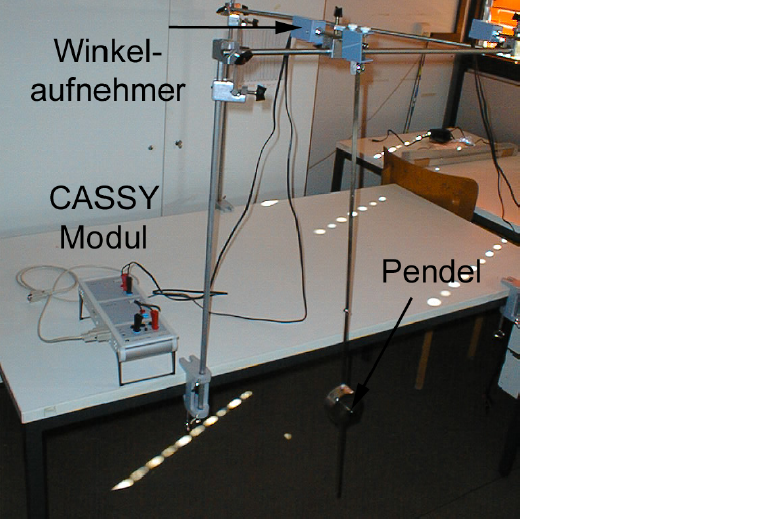
\includegraphics[trim=0 0 6cm 0,clip=True,scale=0.6]{Cassy}
\caption{Versuchsaufbau zur Bestimmung der Erdbeschleunigung}
\label{pic: Cassy}
\end{figure}

\paragraph{Bestimmung der Frequenz}
Um die Periodendauer der aufgezeichneten Schwingung zu bestimmen, zählt man eine bestimmte Anzahl $n$ voller Perioden aus und bildet den Quotienten aus den entsprechenden Zeitintervallen und der Anzahl $n$ 
\begin{equation}
T = \frac{t_2 - t_1}{n}.
\end{equation}
Daraus kann man nun die Kreisfrequenz bestimmen
\begin{equation}
\omega = \frac{2\pi}{T}
\end{equation}
Man sollte entsprechend eine große Anzahl an Perioden nehmen,um eine größere Genauigkeit der Periodendauer zu erhalten.
Der Fehler auf die Periodendauer lautet
\begin{equation}
\sigma_T = \frac{\surd 2 \cdot \sigma_t }{n}
\end{equation}

\subsection{Bestimmung der Erdbeschleunigung}

Zunächst muss die Länge des Pendels - in mehreren Teilen - und der Radius des Pendelkörpers gemessen werden. Dazu misst man zuerst mit dem Messschieber die Länge vom Aufhängepunkt bis zur unteren Kante des Winkelaufnehmers und von das aus mit dem Maßband bis zum Schwerpunkt des Pendelkörpers. Dafür ergibt sich
\begin{equation*}
	l_P = 0.669 \pm 0.001 m \qquad r_P = 4.0 \pm 0.005 cm
\end{equation*}
wobei der Fehler des Maßbandes dominiert. Die Frequenz des Pendels wurde mithilfe der FFT aus der scipy-Bibliothek bestimmt, wie in Abbildung \ref{pic:Einfachpendel} zu sehen ist. 
\begin{equation*}
	\omega = 2\pi f = 2\pi \cdot \left( 0.612 \pm \frac{0.005}{\sqrt{12}} \right) Hz
\end{equation*}
Wie man aus den beiden Fouriertransformationen in den Abbildungen \ref{pic:Einfachpendel} und \ref{pic:Stange} sieht, hat es gut funktioniert die Schwingungen des Pendels mit der Pendelstange anzugleichen.

\begin{figure}[H]
	\centering
	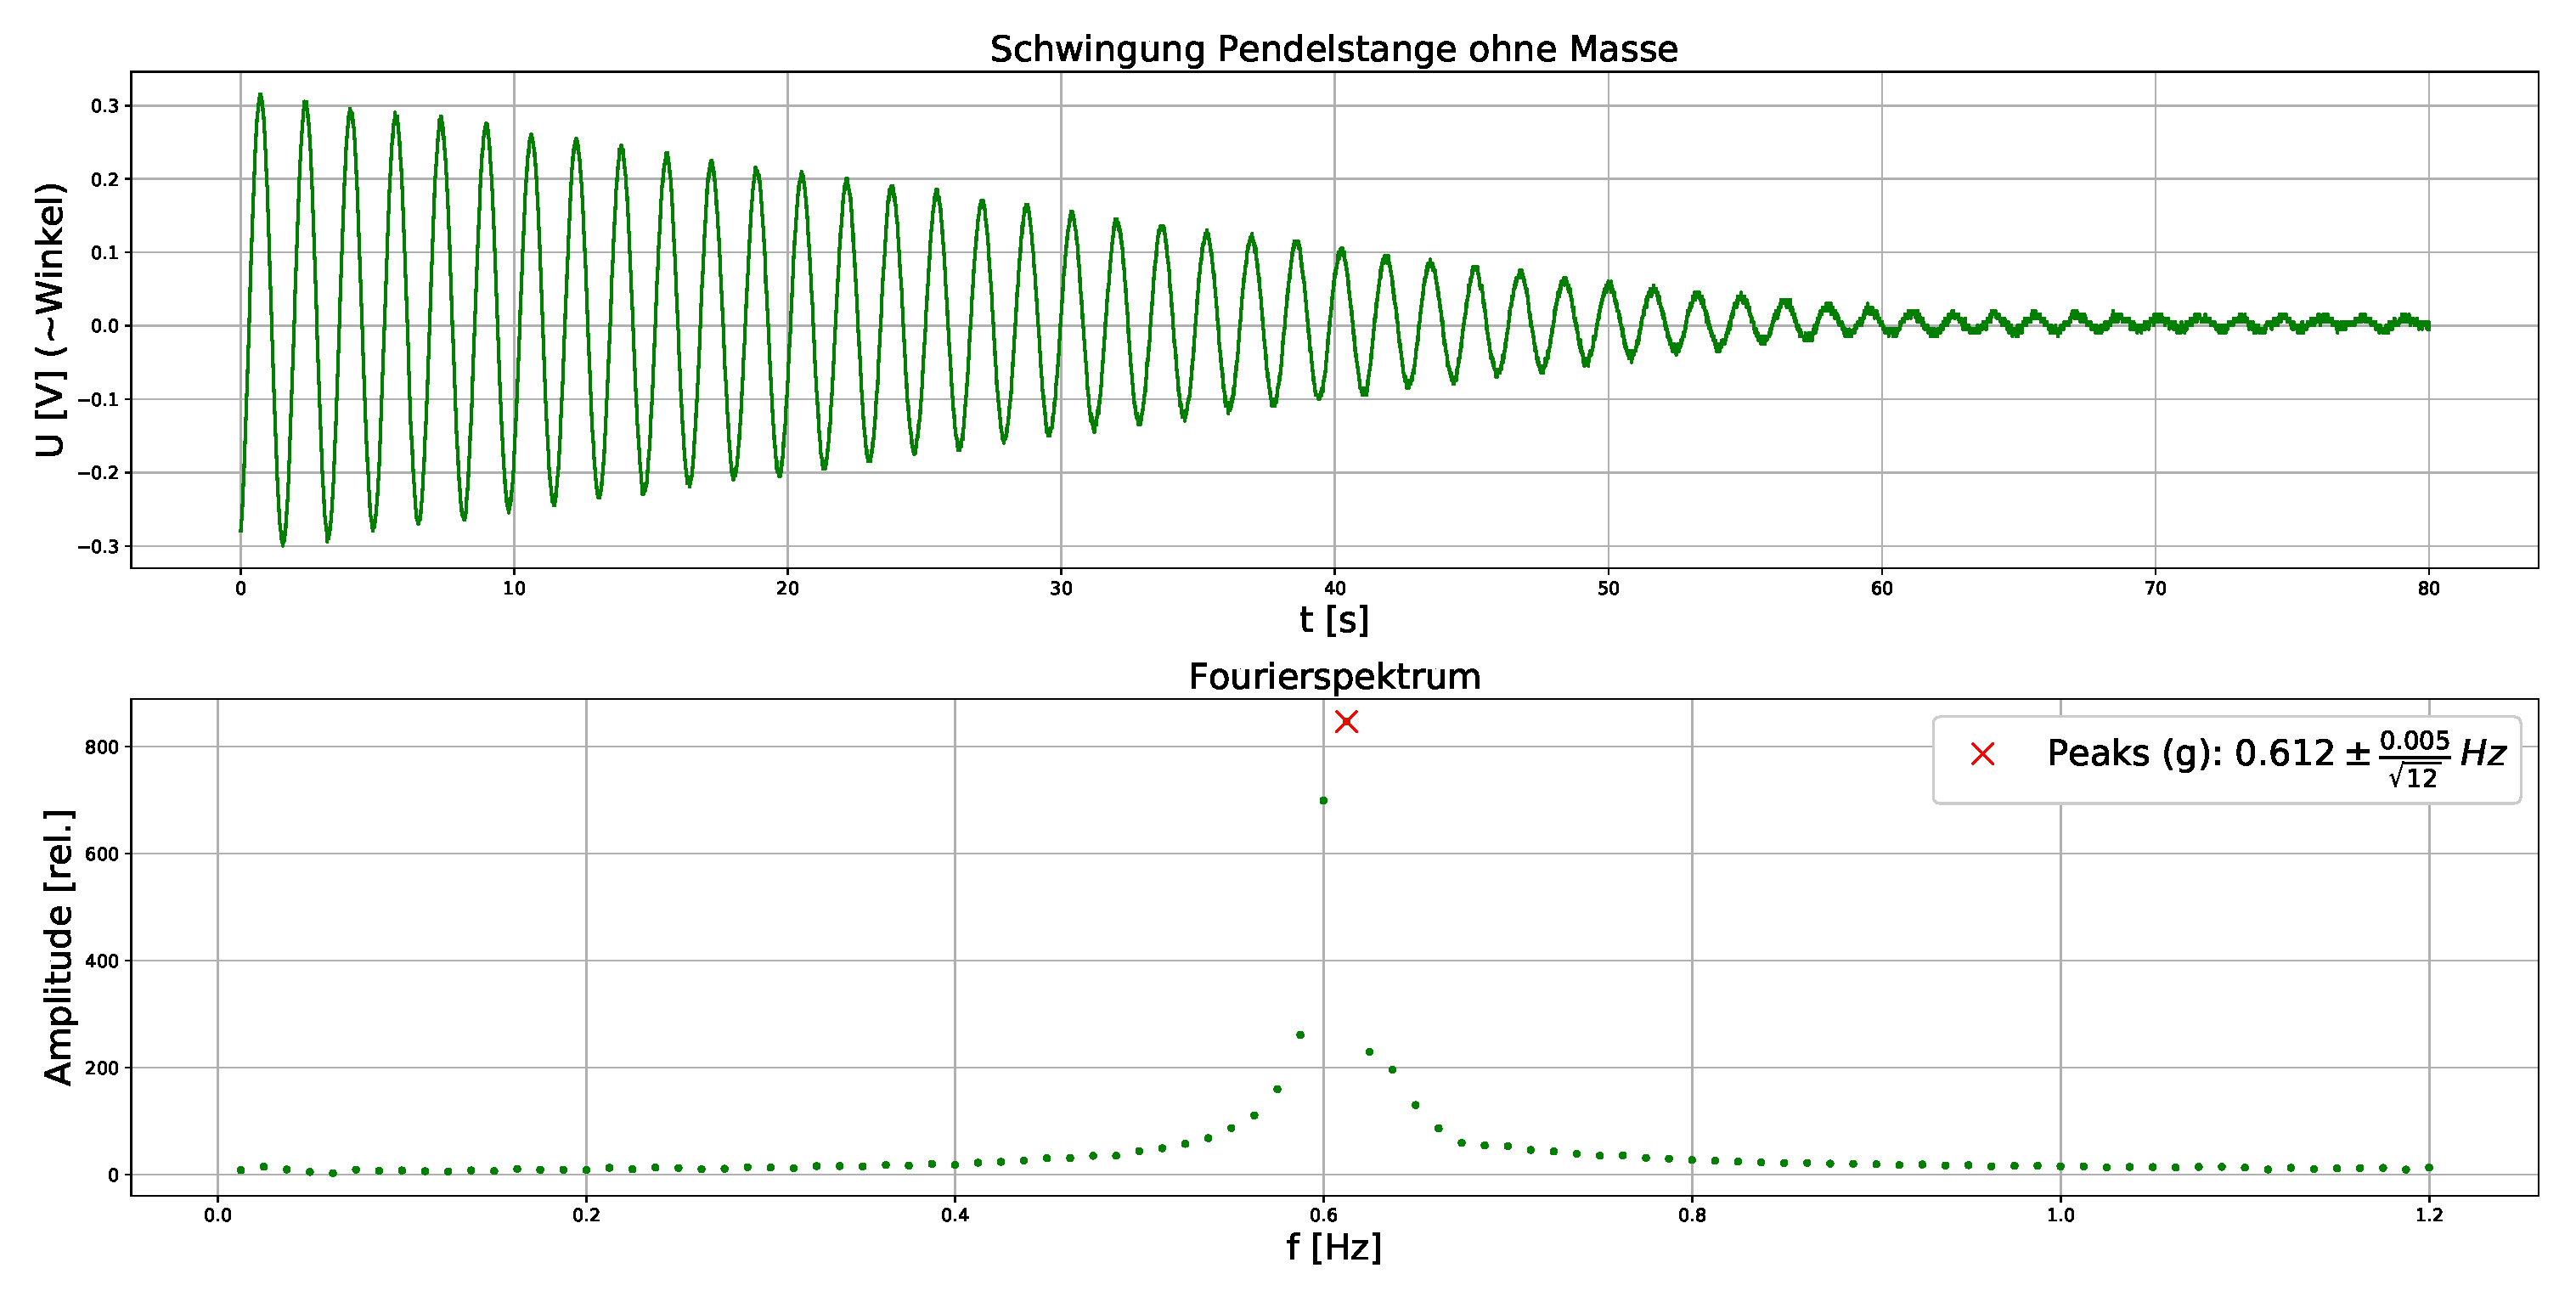
\includegraphics[scale=0.3]{Plots/Stange.eps}
	\caption{Schwingung der Pendelstange ohne Pendelkörper}
	\label{pic:Stange}
\end{figure}
\begin{figure}[H]
	\centering
	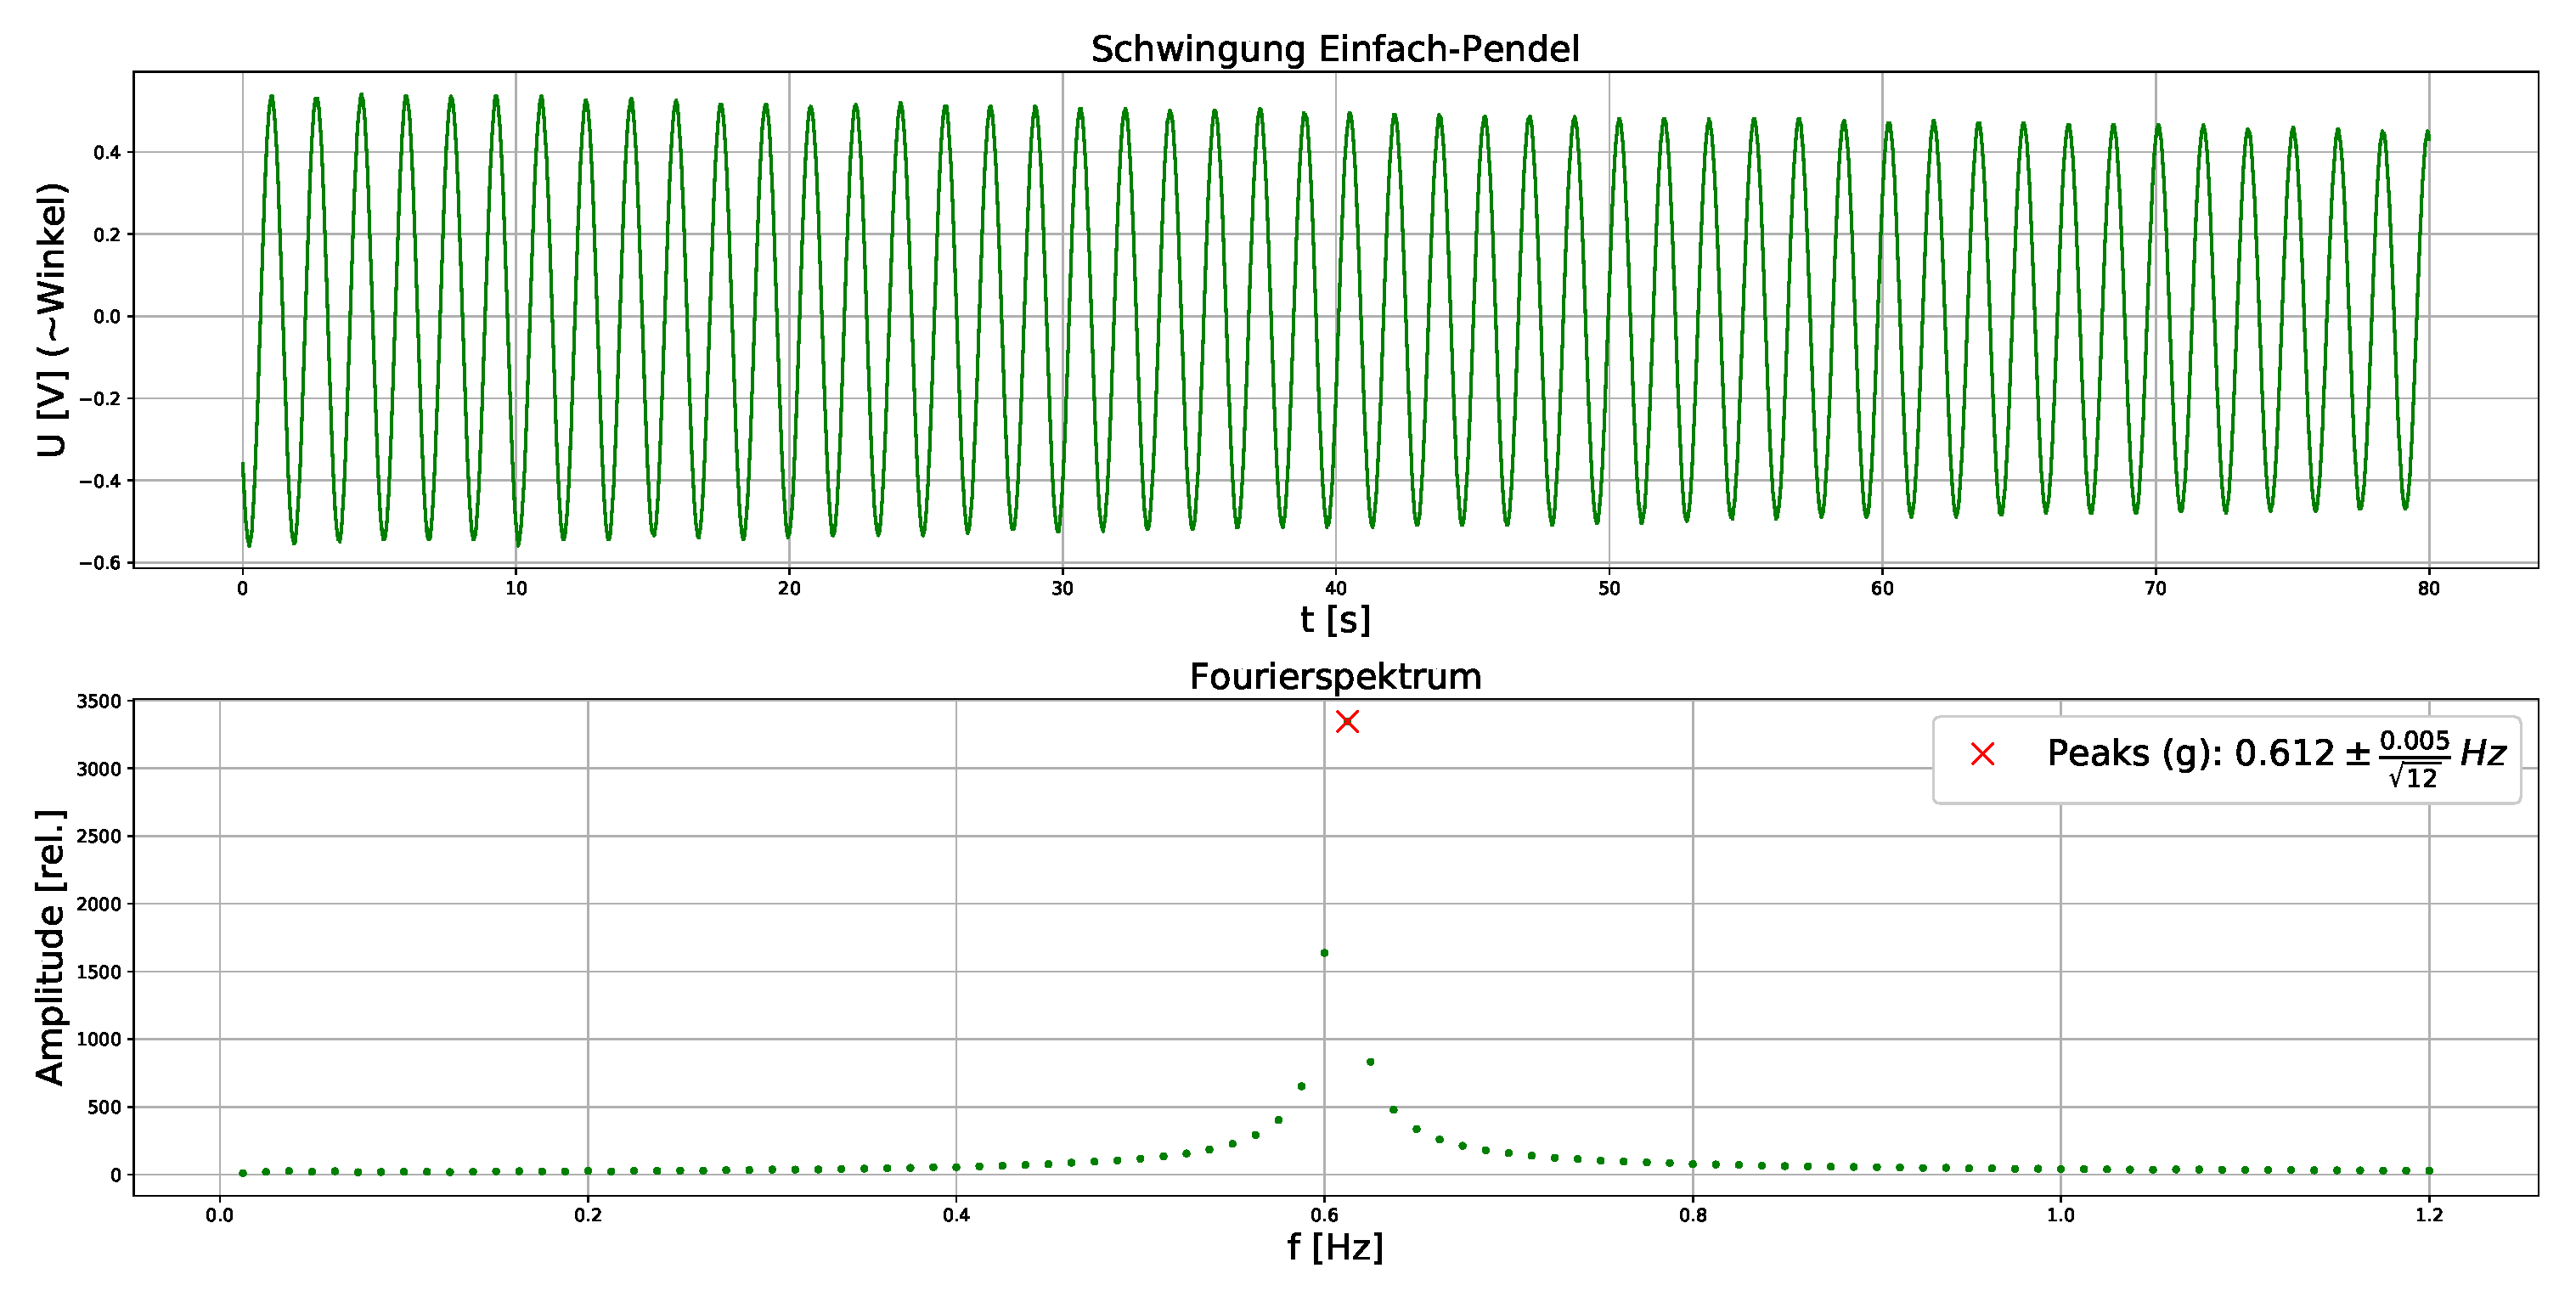
\includegraphics[scale=0.3]{Plots/Einfachpendel.eps}
	\caption{Schwingung eines Pendels mit Pendelkörper}
	\label{pic:Einfachpendel}
\end{figure}


Daraus kann dann $g$ berechnet werden: 
\begin{equation*}
g = \omega^2 \cdot l_P \cdot (1+\frac{r_P^2}{2 \cdot l_P^2})   
\end{equation*}


Für den Fehler auf $g$ lautet das Fehlerfortpflanzungsgesetz:
\begin{equation*}
\sigma_g = \frac{\partial g}{\partial T}\cdot\sigma_T \oplus \frac{\partial g}{\partial l}\cdot\sigma_l \oplus \frac{\partial g}{\partial r}\cdot\sigma_r = \sqrt{\left(\frac{\partial g}{\partial T}\cdot\sigma_T\right)^2 + \left( \frac{\partial g}{\partial l}\cdot\sigma_l\right)^2+\left( \frac{\partial g}{\partial r}\cdot\sigma_r\right)^2} 
\end{equation*}\
Es werden nun die Summanden separat betrachtet, um abzuschätzen, welche Größe am meisten zum Fehler beiträgt:
\begin{equation*}
\left(\frac{\partial g}{\partial \omega}\cdot\sigma_{\omega}\right)^2 = 2,151 \cdot 10^{-3} \frac{m^2}{s^4} 
\end{equation*}
\begin{equation*}
\left(\frac{\partial g}{\partial r}\cdot\sigma_r\right)^2 = 1,8988 \cdot 10^{-11} \frac{m^2}{s^4} 
\end{equation*}
\begin{equation*}
\left(\frac{\partial g}{\partial l}\cdot\sigma_l\right)^2 = 2,11898 \cdot 10^{-4} \frac{m^2}{s^4}
\end{equation*}
\begin{equation*}
\Rightarrow \sigma_g = 0,0486 \frac{m}{s^2}
\end{equation*}\
Damit ergibt sich eine Erdbeschleunigung von
\begin{equation}
g = 9,786 \pm0,049 \frac{m}{s^2}
\end{equation}


\subsection{Fazit}
Der Versuch zur Bestimmung der Erdbeschleunigung hat im Allgemeinen gut geklappt. Die einzige Schwierigkeit bestand darin, die richtige Frequenz mittels der FFT zu bestimmen (den Peak zu finden) und Präzise bei der Längenmessung zu sein. 

Der Literaturwert für die Erdbeschleunigung liegt bei $g = 9,81 \frac{m}{s^2}$. Damit ist unser gemessener Wert in einer $0,49\, \sigma$ Umgebung. 

\clearpage
\section{Schwingungen von gekoppelten Pendeln}
\subsection{Grundlagen}
Ein gekoppeltes Pendel besteht aus zwei Pendeln, die durch eine Kopplungsfeder miteinander verbunden sind. Die physikalischen Pendel werden dabei so angebracht, dass sie die Feder spannt, d.h. die hängen im Gleichgewicht nicht vertikal runter, sondern sind um einen Winkel $\phi$ nach innen verschoben. Das dadurch erzeugte Drehmoment, bewirkt durch die Feder, lautet
\begin{equation}
M_F = -D_F \cdot x_0 \cdot l_F.
\end{equation}  
Dabei beschreit $D_F$ die Federkonstante und $x_0$ die Verlängerung gegenüber der entspannten Feder. Im Ruhezustand ist das durch die Feder erzeugte Drehmoment entgegengesetzt gleich dem Drehmoment, dass durch die Schwerkraft erzeugt wird
\begin{equation}
M_S = m \cdot g \cdot l_S \cdot \phi_O.
\end{equation}
Dabei beschreibt $l_S$ die Entfernung des Schwerpunktes der Pendel zu seiner Drehachse und $\phi_0$ der Winkel, der entsteht, wenn das Pendel in der Ruhelage, aufgrund der Spannung der Feder, nach innen ausgelenkt wird.
Das resultierende Drehmoment auf Pendel 1 lautet
\begin{equation}
M_1 = J \cdot \ddot \phi_1 = -m \cdot g \cdot l_S \cdot \phi_1 - D_F \cdot l_F^2 \cdot (\phi_2 - \phi_1)
\end{equation}
\begin{equation}
M_2 = J \cdot \ddot \phi_2 = -m \cdot g \cdot l_S \cdot \phi_2 - D_F \cdot l_F^2 \cdot (\phi_2 - \phi_1)
\end{equation} 
Die Bewegungsgleichungen lauten für die Anfangsbedingungen $\dot \phi_1(0) = 0$ und $\dot \phi_2(0) = 0$  
\begin{equation}
2\phi_1(t) = B \cdot cos(\omega_s t) - D \cdot cos(\omega_{sf} t)
\end{equation}
\begin{equation}
2\phi_2(t) = B \cdot cos(\omega_s t) - D \cdot cos(\omega_{sf} t)
\end{equation}

%\begin{figure}[H]
%\centering
%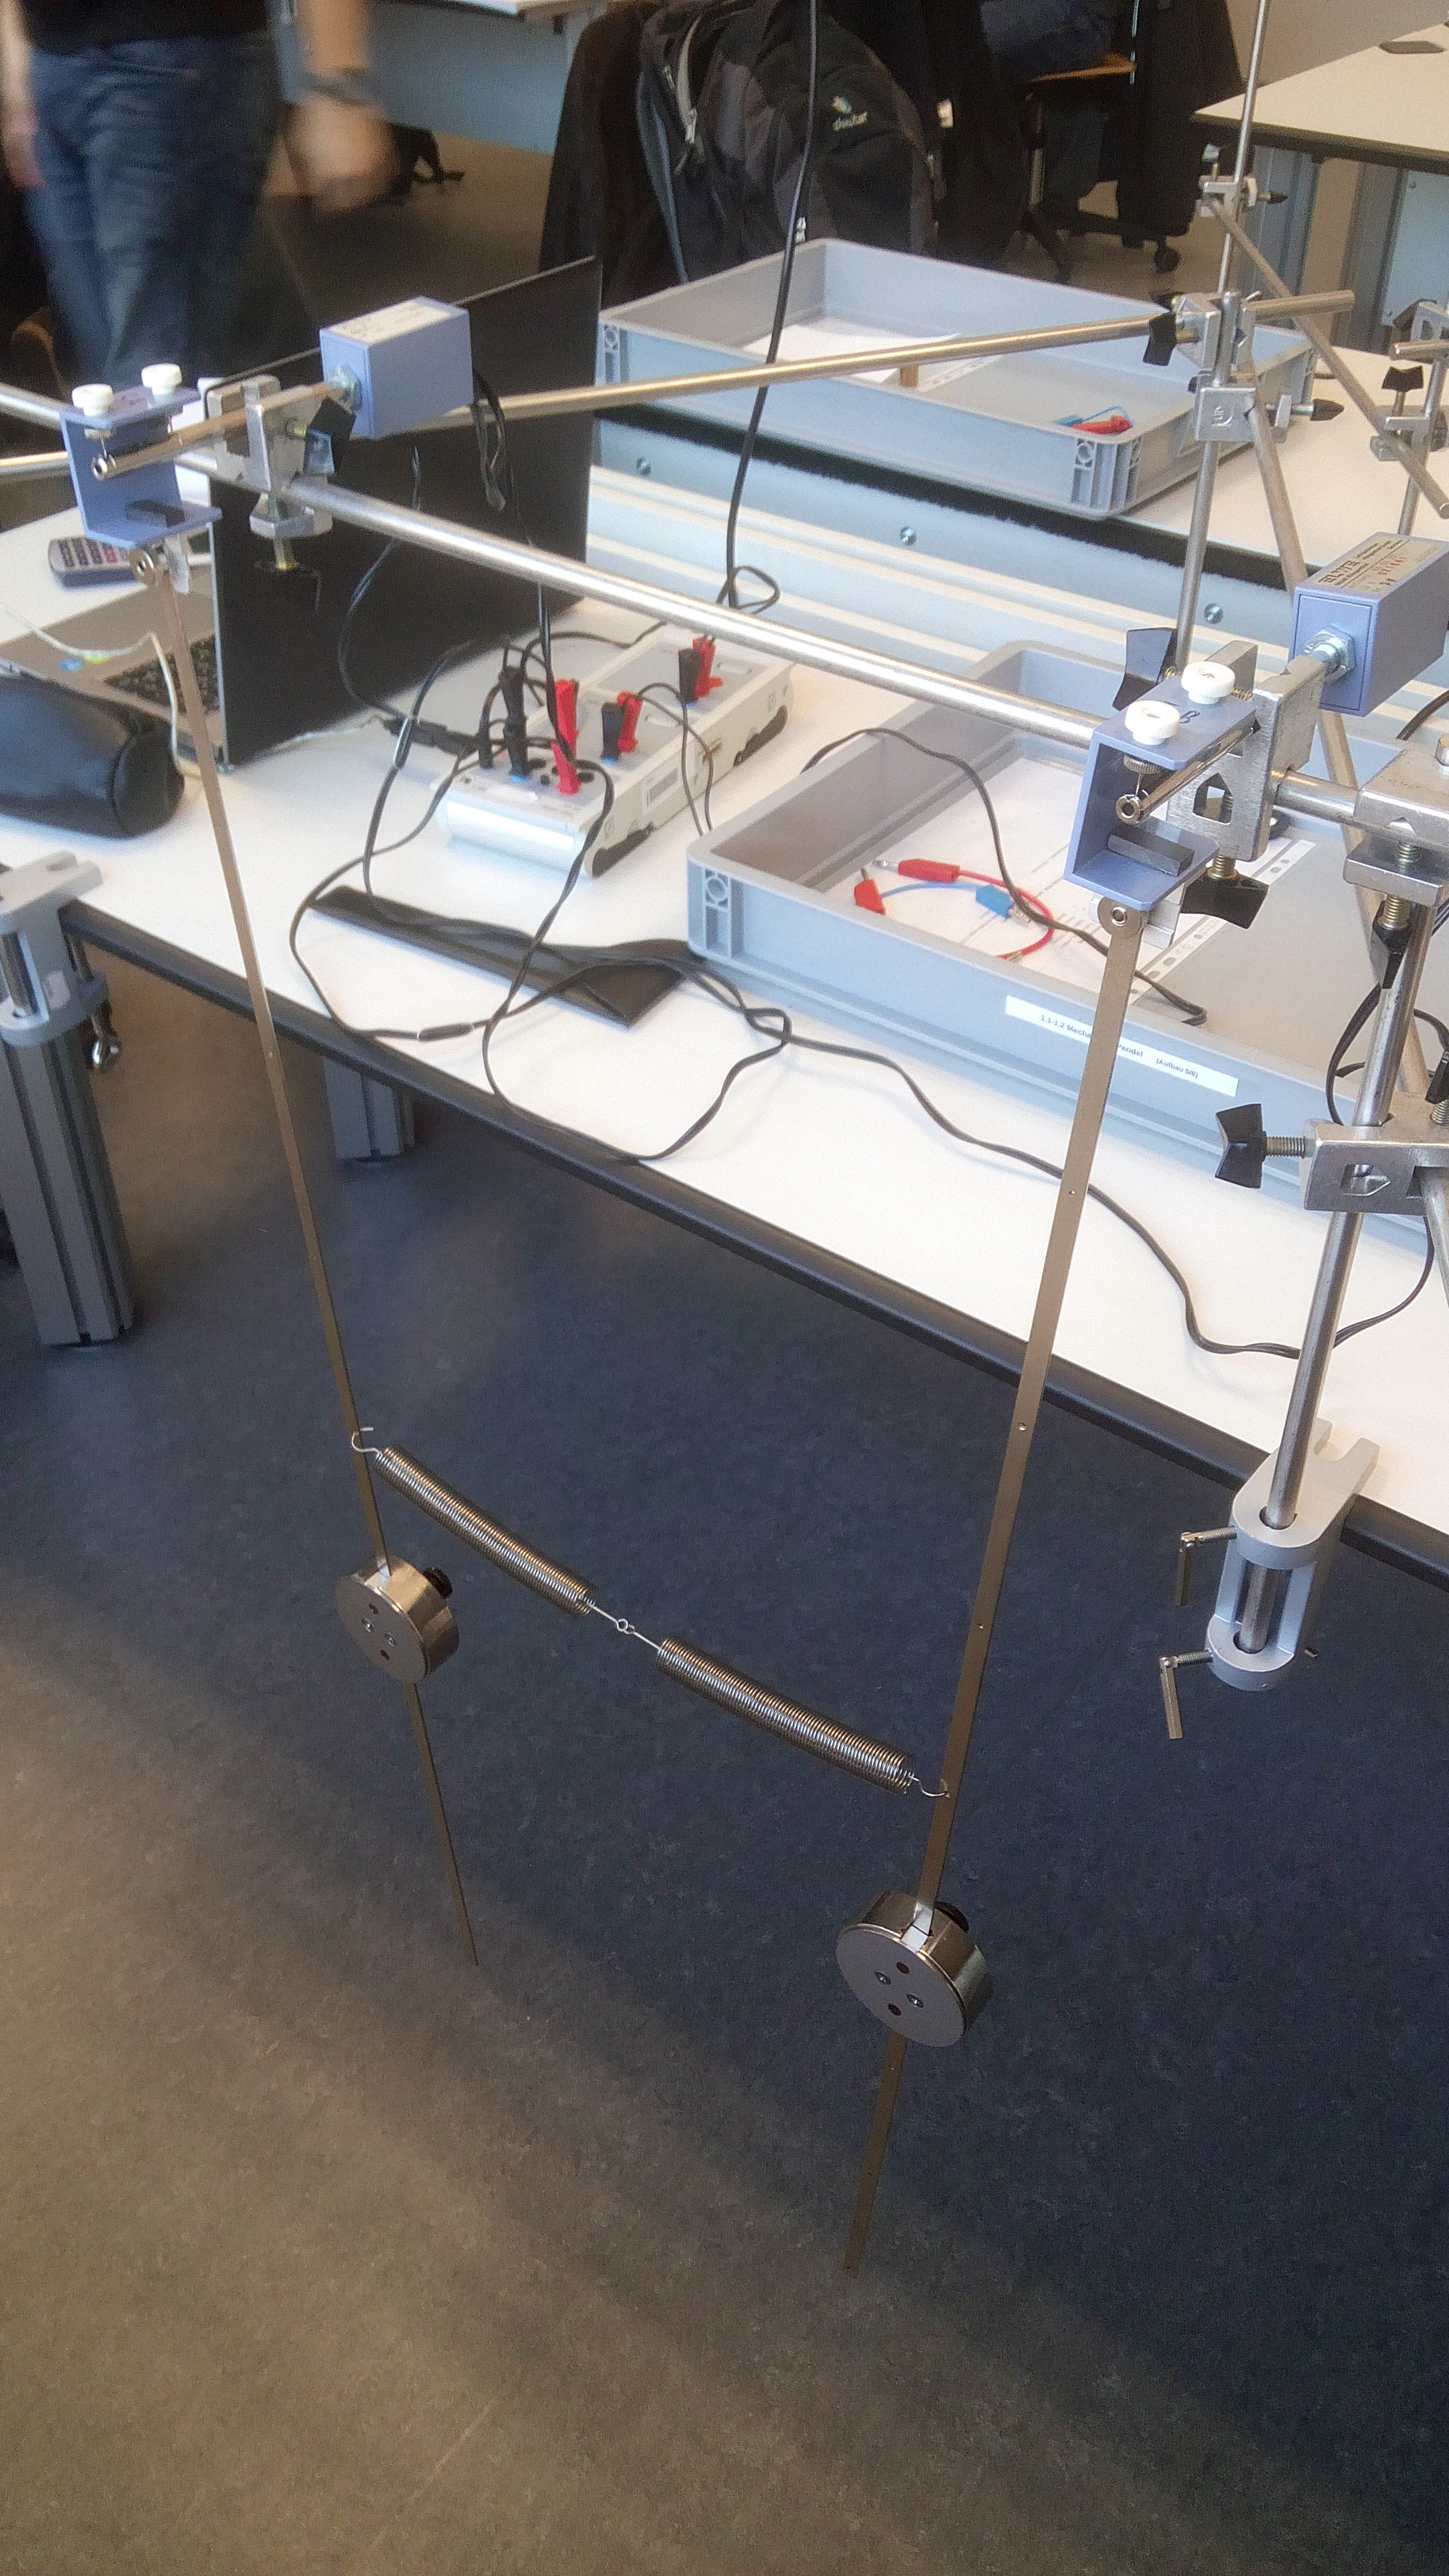
\includegraphics[scale=0.5]{Doppelpendel}
%\caption{Zwei Pendel, die über eine Feder miteinander gekoppelt sind}
%\label{pic: gekoppelte Doppelpendel}
%\end{figure}

Nun gibt es 3 Fälle zu betrachten

\begin{enumerate}
	\item gleichsinnige Schwingung, wenn $\phi_1(0) = \phi_{max}$ und $\phi_2(0) = \phi_{max}$
	\begin{equation}
	\phi_1(t) = \phi_{max} \cdot cos(\omega_S t)
	\end{equation}  
	\begin{equation}
	\phi_2(t) = \phi_{max} \cdot cos(\omega_S t),
	\end{equation}
	wobei $\omega_S = \frac{mgl_S}{J}$ die Kreisfrequenz ist, die durch die Schwerkraft erzeugt wird
	
	\item gegensinnige Schwingung, wenn $\phi_1(0) = -\phi_{max}$ und $\phi_2(0) = \phi_{max}$
	\begin{equation}
	\phi_1(t) = \phi_{max} \cdot cos(\omega_{Sf} t)
	\end{equation}
	\begin{equation}
	\phi_2(t) = -\phi_{max} \cdot cos(\omega_{Sf} t),
	\end{equation}
	wobei $\omega_{Sf}^2 = \omega_S^2 + 2\Omega^2$ und $\Omega = \frac{D_Fl_F^2}{J}$ die Kreisfrequenz, die durch die Federkraft erzeugt wird.
	
	\item Überlagerung von zwei verschiedenen Frequenzen, wenn $\phi_1(0) = \phi_{max}$ und $\phi_2(0) = 0$
	\begin{equation}
	\phi_1(t) = \phi_{max} \cdot cos(\omega_{sch} t)cos(\omega_k t)
	\end{equation}
	\begin{equation}
	\phi_2(t) = \phi_{max} \cdot \cos(\omega_{sch} t)\cos(\omega_k t),
	\end{equation}
	wobei $\omega_{sch} = \frac{\omega_{Sf} - \omega_S}{2}$ und $\omega_k = \frac{\omega_{Sf} + \omega_S}{2}$
\end{enumerate}

Mit den nun bestimmten Größen kann man im Folgenden die Schwingungsdauern zu den verschiedenen Fällen bestimmen, sowie den Kopplungsgrad der Feder. Für die gleichsinnige Schwingung ergibt sich die Schwingungsdauer
\begin{equation}
T_S = \frac{2\pi}{\omega_S},
\end{equation}
für die gegensinnige Mode 
\begin{equation}
T_{Sf} = \frac{2\pi}{\omega_{Sf}}
\end{equation}
und für die Schwebung
\begin{equation}
T_k = \frac{2\pi}{\omega_k} = \frac{4\pi}{\omega_S + \omega_{Sf}}
\end{equation}
und 
\begin{equation}
T_{sch} = \frac{2\pi}{\omega_{sch}} = \frac{4\pi}{\omega_{sf} - \omega_S}.
\end{equation}

Für den Kopplungsgrad ergibt sich 
\begin{equation}\label{eq:kappa}
\kappa = \frac{\Omega^2}{\omega_S^2 + \Omega^2} = \frac{D_F l_F^2}{mgl_s + D_F l_F^2 } \quad \Rightarrow \quad D_F = \frac{mgl_s}{\left(\frac{1}{\kappa}-1\right) l_F^2 } 
\end{equation}


\subsection{Aufbau und Durchführung}
Der Aufbau ähnelt dem Aufbau zur Bestimmung der Erdbeschleunigung. Es werden zwei Pendel in einem bestimmten Abstand auf einem Drei-Bein-Gestell aufgehängt und über eine Feder gekoppelt. Dadurch, dass die Federn nicht gestaucht werden können, müssen die Pendel so weit voneinander entfernt sein, dass die Feder in der Ruhelage gespannt ist. Die Auslenkwinkel der beiden Pendel kann wieder, wie im ersten Versuch, über einen Winkelaufnehmer gleichzeitig über ein Cassy-Modul ausgelesen werden. Es muss darauf geachtet werden, beide der Auslenkung Pendel diese in einer Ebene zu lassen, um Schwingungen in Querrichtung zu vermeiden.

\subsection{Auswertung}

\subsubsection{Gleichsinnige Schwingung}
\begin{figure}[H]
	\centering
	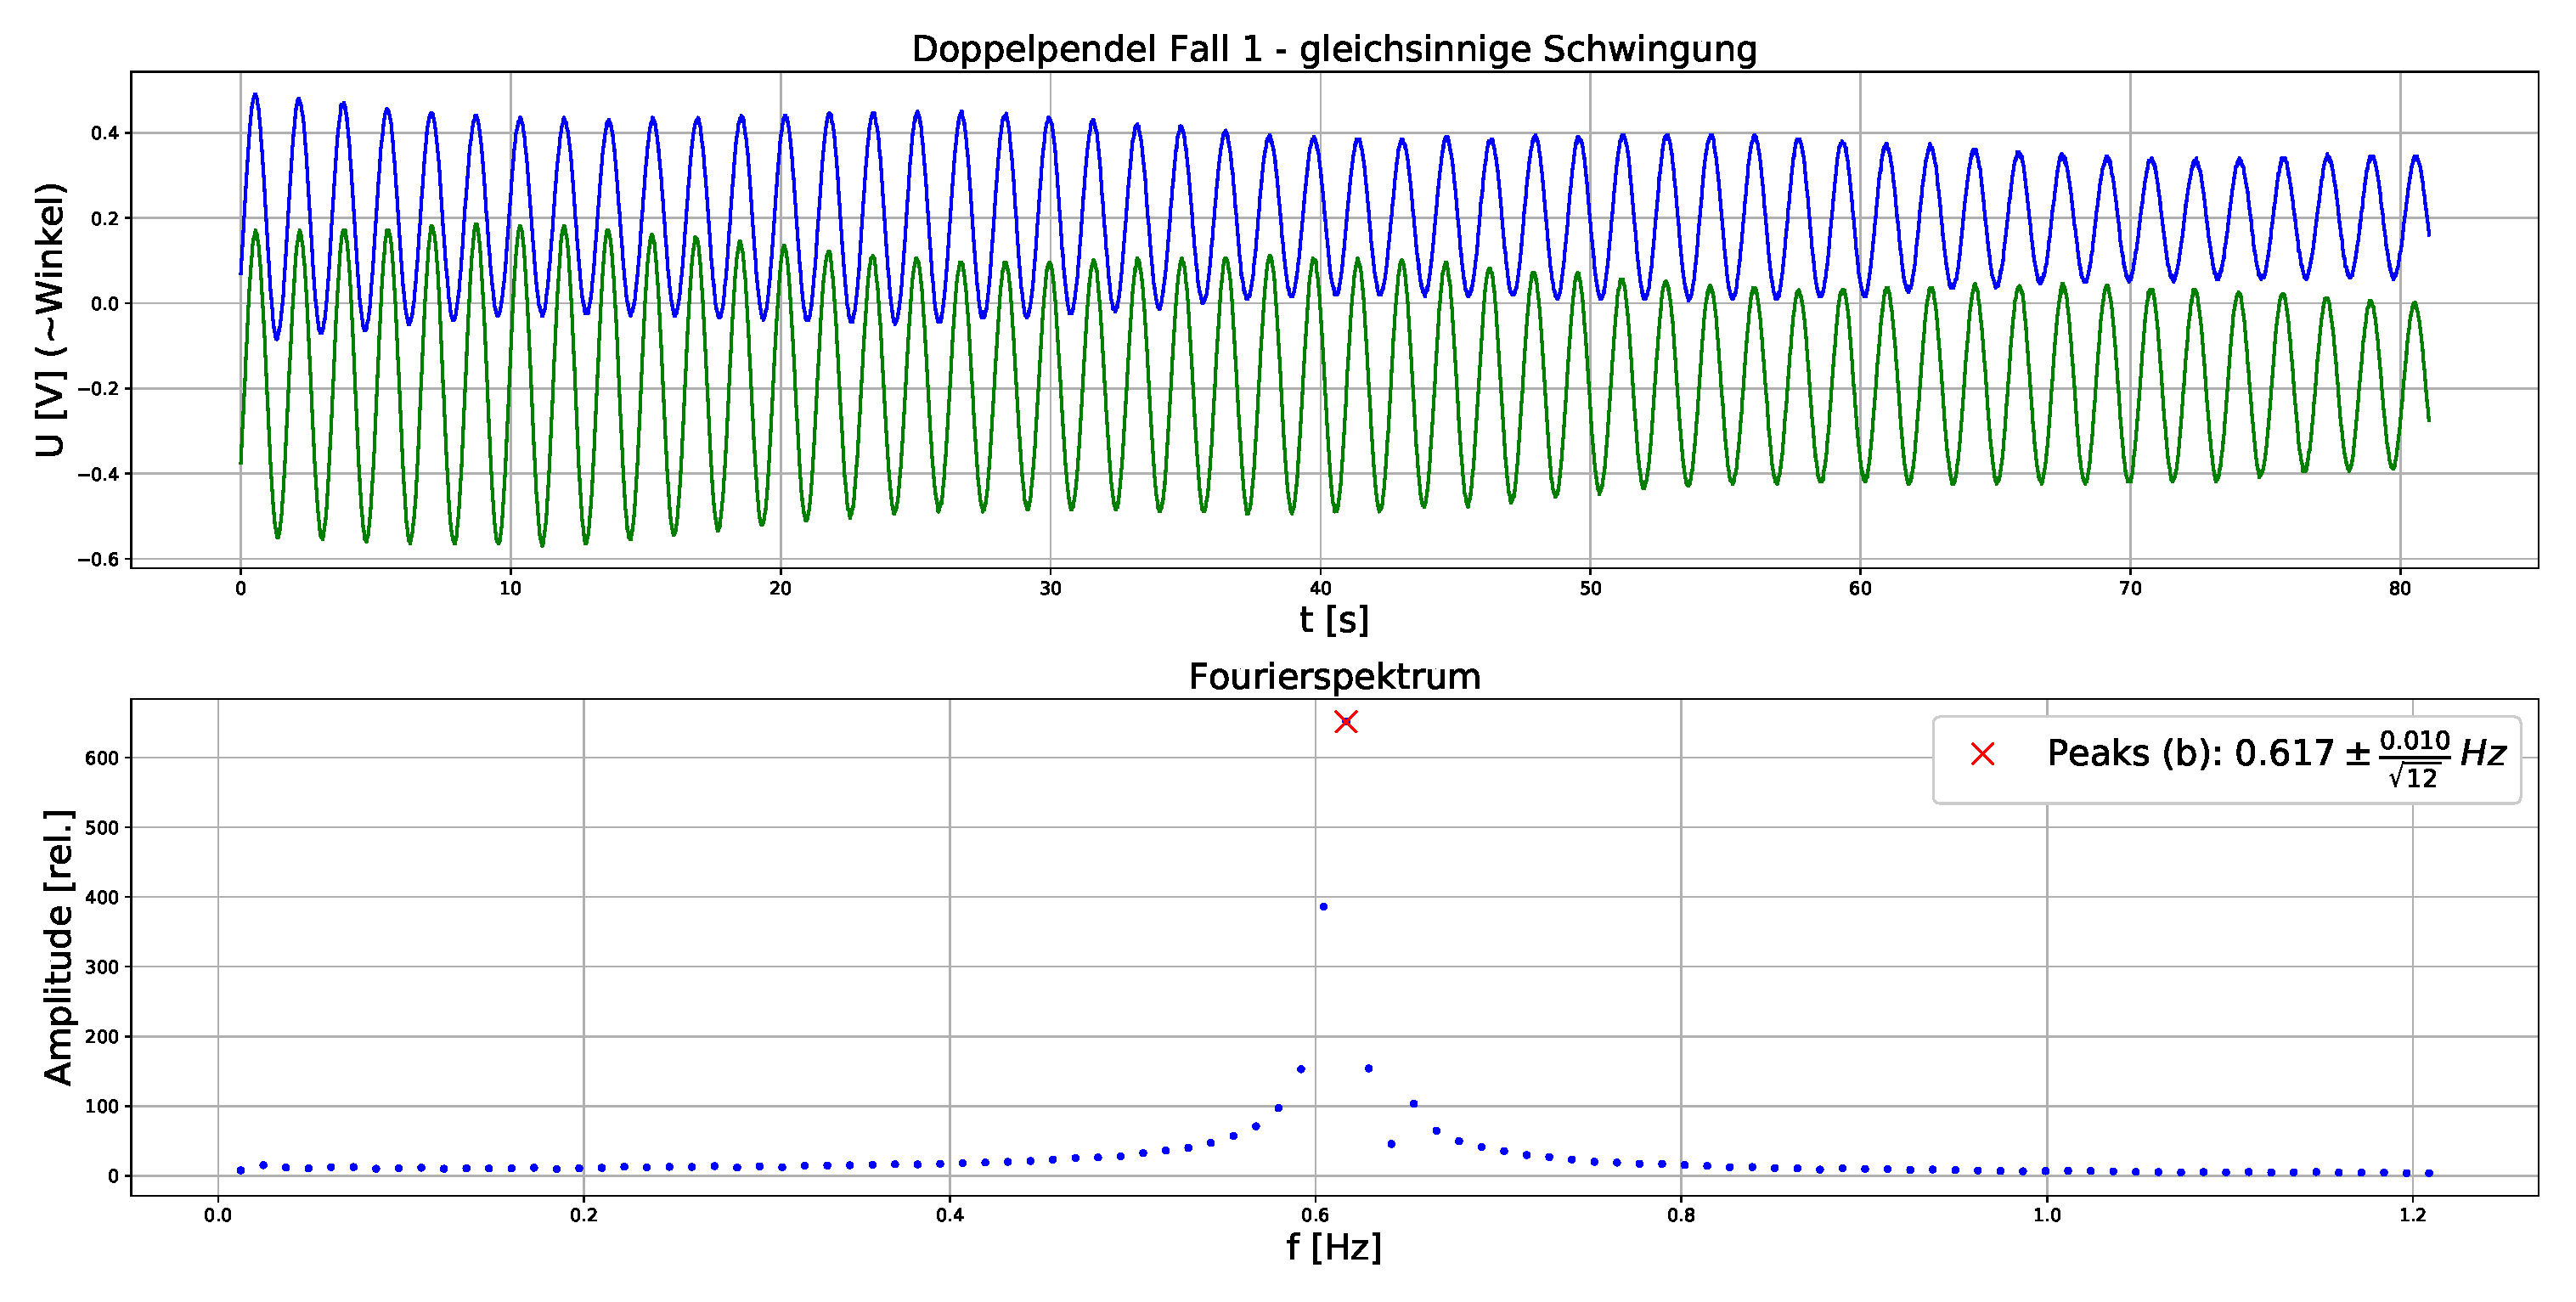
\includegraphics[scale=0.3]{Plots/Doppelpendel1.eps}
	\caption{Gleichsinnige Schwingung des Doppelpendels}
	\label{pic:Doppelpendel1}
\end{figure}
Mit Hilfe der FFT wird die Frequenz $\omega_s$ der gleichsinnigen Schwingung (ohne Kopplung) bestimmt:
\begin{equation*}
	\omega_s = 2\pi f_s = 2\pi \cdot \left( 0.617 \pm \frac{0.01}{\sqrt{12}} \right) Hz
\end{equation*}
Wie oben wird hier für den Fehler auf die mit einer Peakfinder-Routine bestimmten Peaks die Gleichverteilung auf der Intervallbreite angenommen.

\subsubsection{Gegensinnige Schwingung}
\begin{figure}[H]
	\centering
	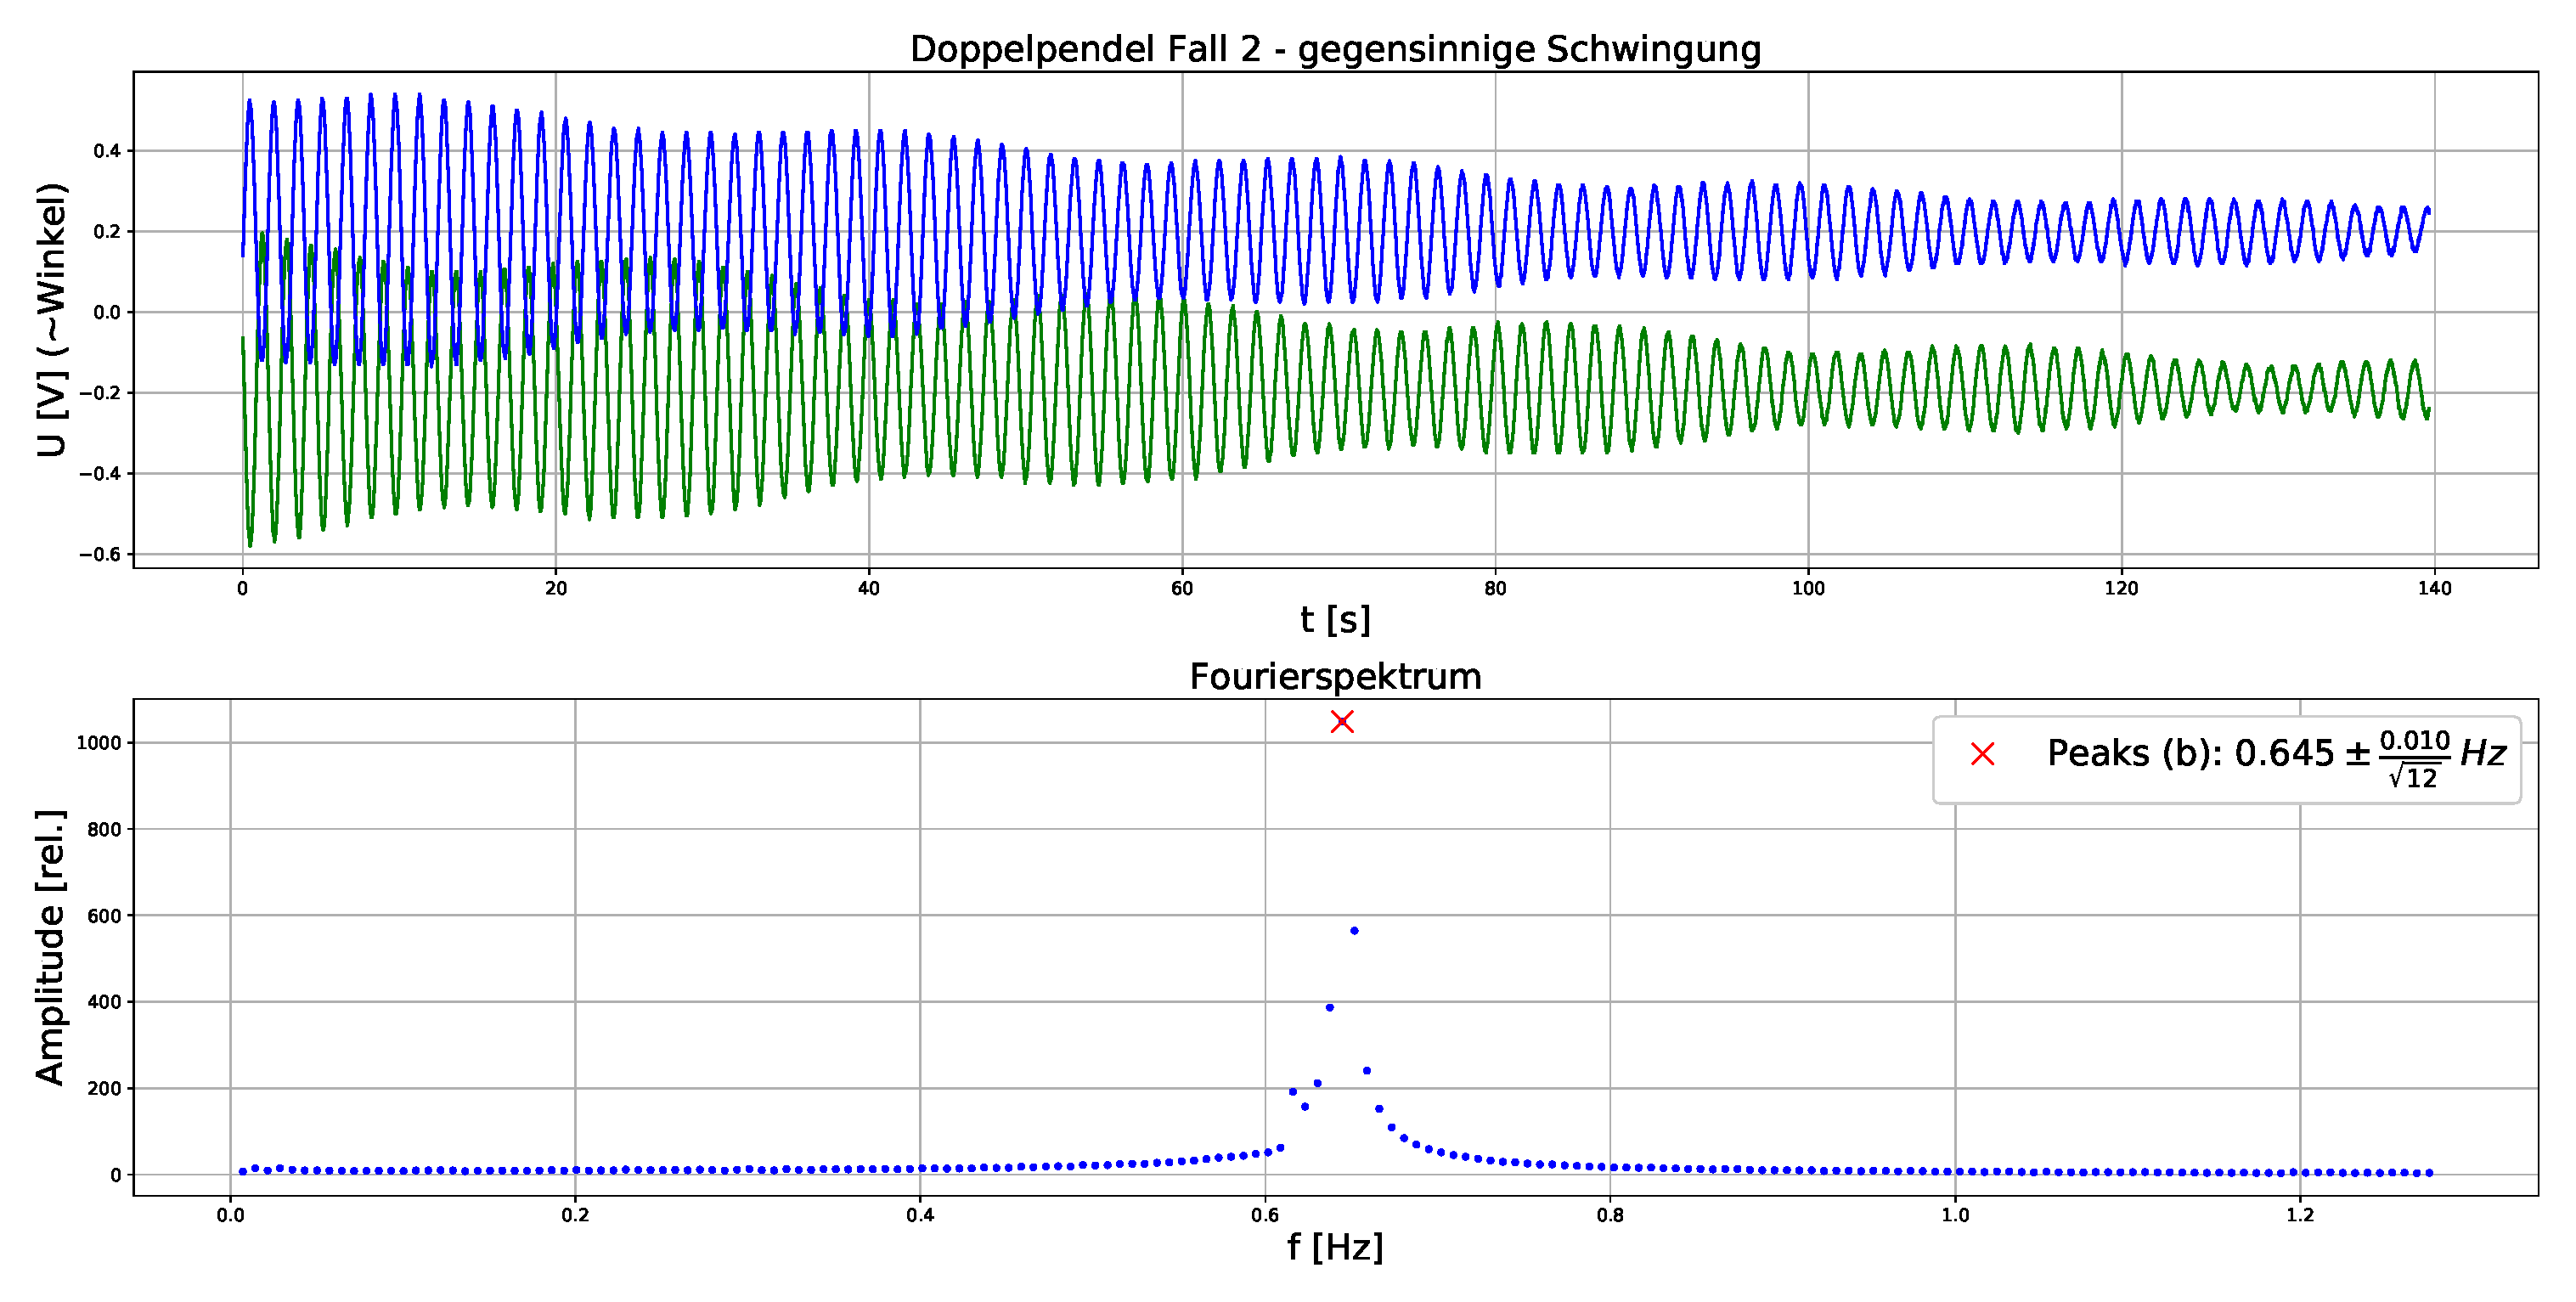
\includegraphics[scale=0.3]{Plots/Doppelpendel2.eps}
	\caption{Gegensinnige Schwingung des Doppelpendels}
	\label{pic:Doppelpendel2}
\end{figure}
Bei der gegensinnigen Schwingung ergibt sich für die Frequenz 
\begin{equation*}
\omega_{sf} = 2\pi f_{sf} = 2\pi \cdot \left( 0.645 \pm \frac{0.01}{\sqrt{12}} \right) Hz
\end{equation*}
Damit kann dann $\Omega$ berechnet werden
\begin{equation}
\Omega = \sqrt{\frac{\omega_{sf}^2-\omega_s^2}{2}} = 0.835 Hz \qquad \sigma_{\Omega} = \sqrt{ \frac{1}{4} \left(\frac{\omega_{sf}^2-\omega_s^2}{2}\right)^{-1} (\omega_{sf}^2+\omega_s^2) } \cdot \frac{0.01}{\sqrt{12}} = 0.009 Hz
\end{equation} 


\subsubsection{Schwebung}
\begin{figure}[H]
	\centering
	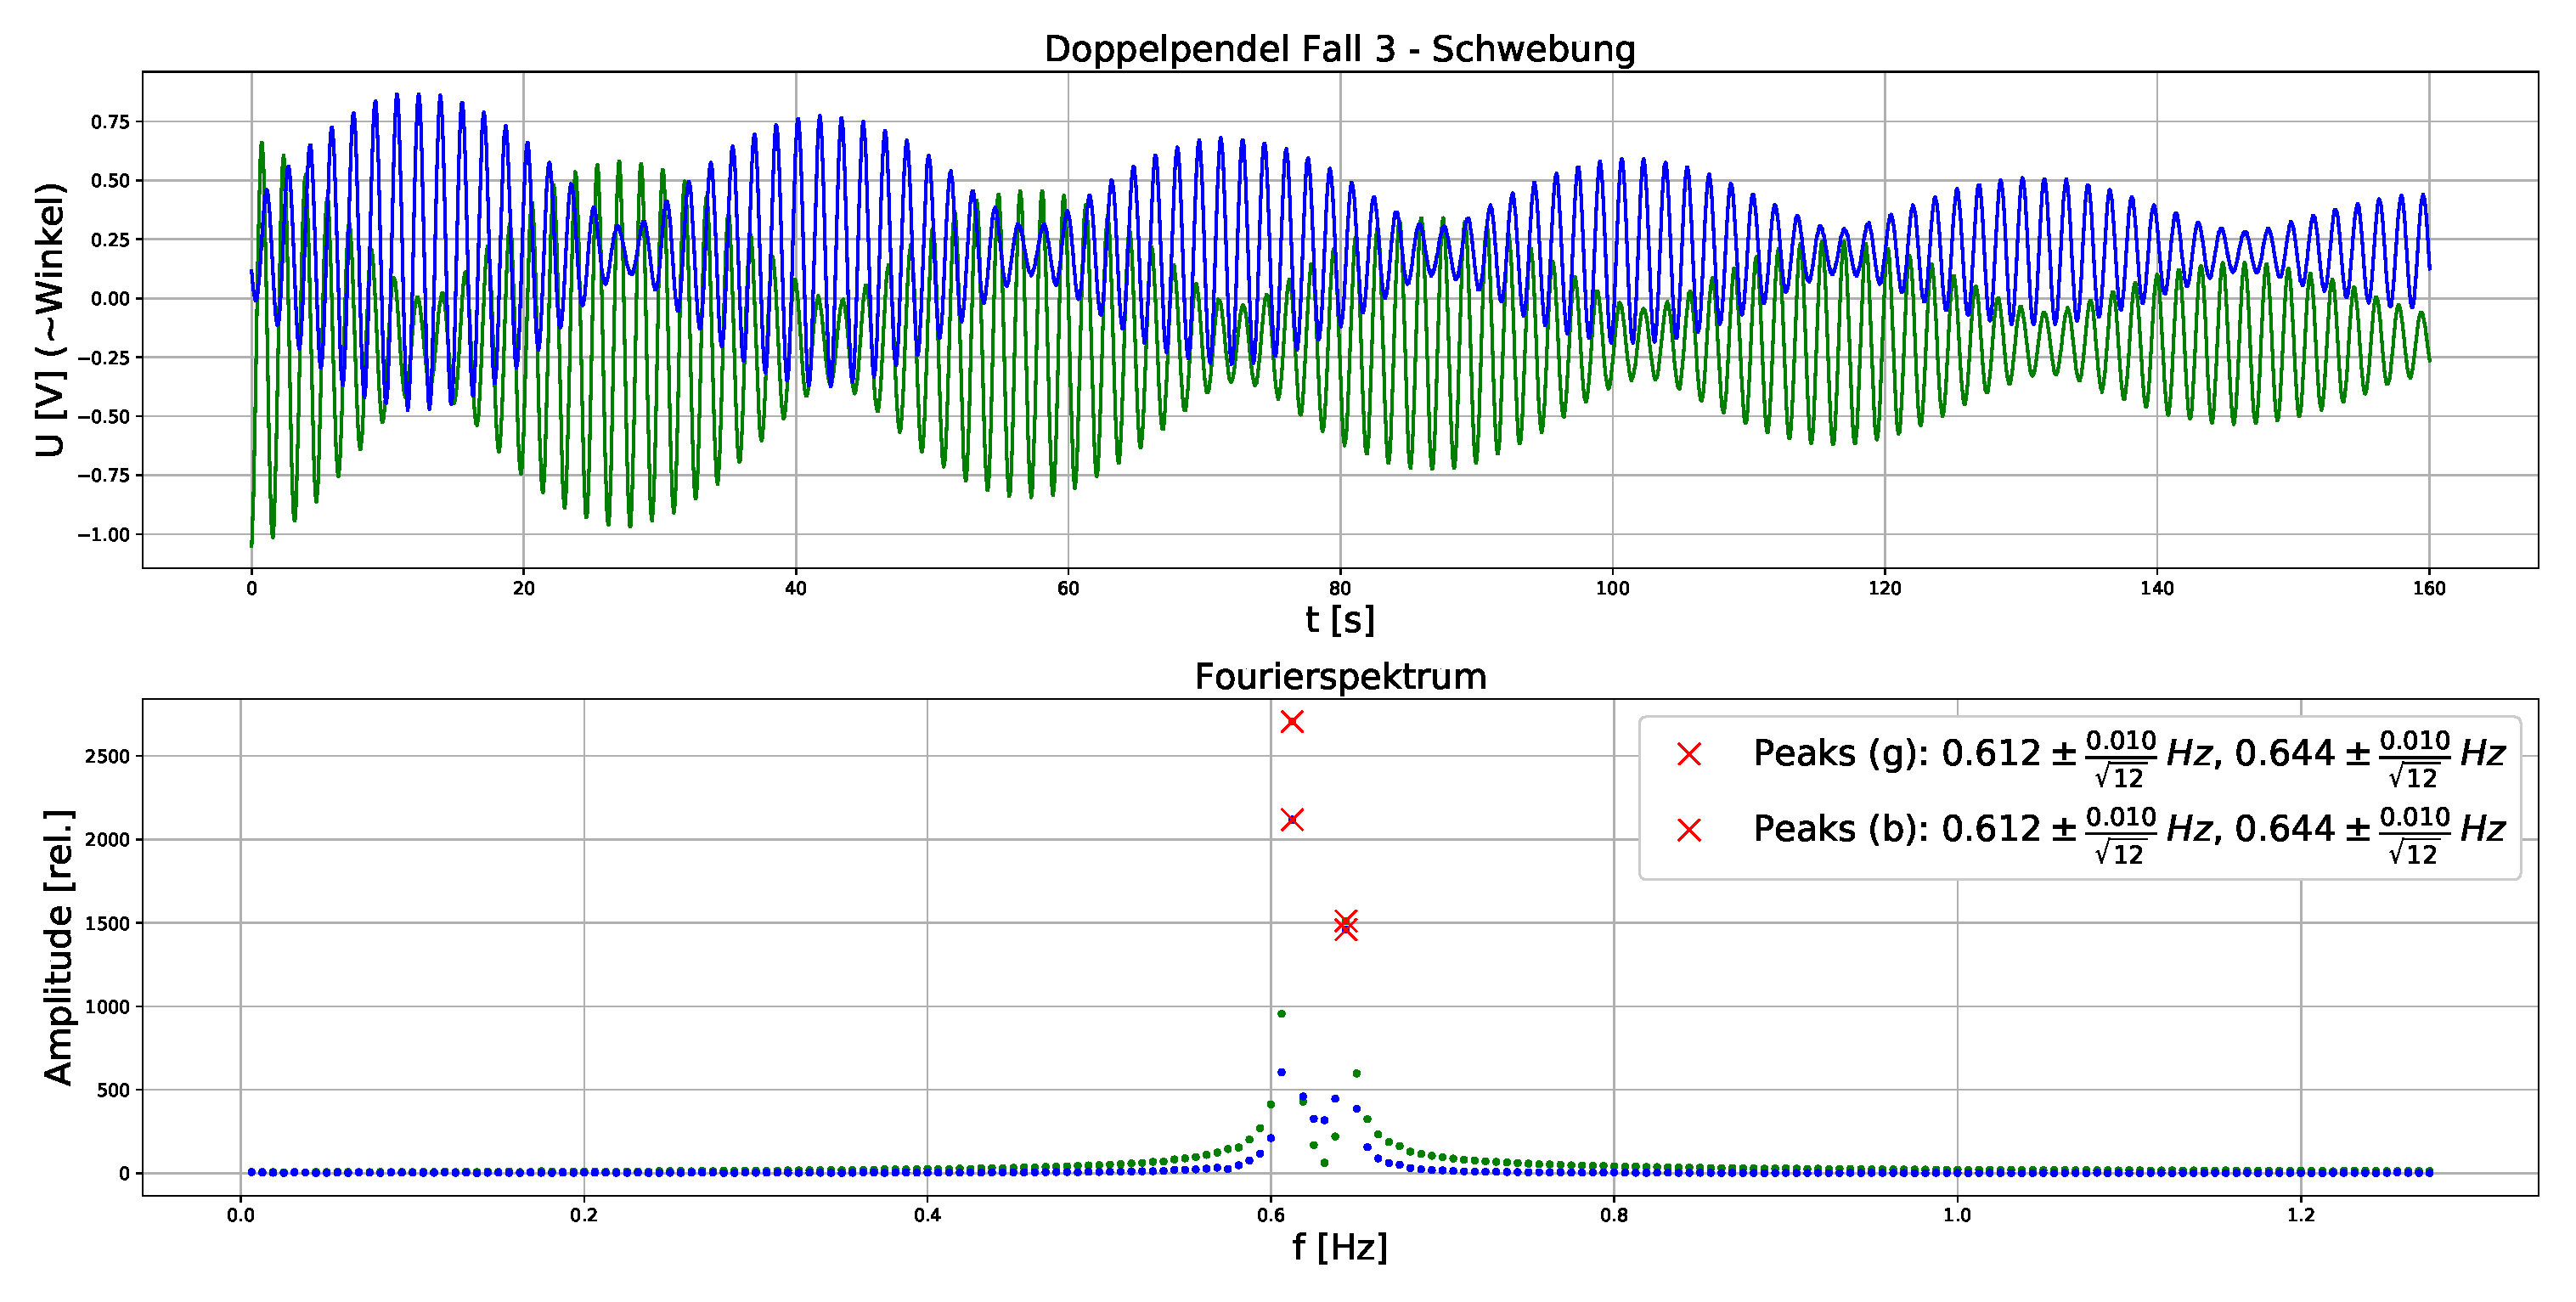
\includegraphics[scale=0.3]{Plots/Doppelpendel3.eps}
	\caption{Schwebung des Doppelpendels}
	\label{pic:Doppelpendel3}
\end{figure}
Bei der Überlagerung zweier Schwingungen ergeben sich aus der FFT die Frequenzen der inneren und äußeren Schwingung (gleich für linkes und rechtes Pendel)
\begin{equation*}
\omega_{k} = 2\pi f_k = 2\pi \cdot \left( 0.644 \pm \frac{0.01}{\sqrt{12}} \right) Hz  \qquad  \omega_{sch} = 2\pi f_{sch} = 2\pi \cdot \left( 0.612 \pm \frac{0.01}{\sqrt{12}} \right) Hz
\end{equation*}


\subsubsection{Bestimmung der Federkonstante}
Mit den ermittelten Frequenzen lässt sich nun der Kopplungsgrad des Pendelsystems mit Hilfe von Gleichung \ref{eq:kappa} bestimmen
\begin{equation}
\kappa = \frac{\Omega^2}{\omega_s^2 + \Omega^2} = 0.0462 \qquad \sigma_{\kappa} = \sqrt{ \left( \left(\frac{\omega_s}{\Omega}\right)^2 + 1 \right)^{-4} \cdot \left(\frac{4\omega_s^2}{\Omega^4}\sigma_{\omega_s}^2 + \frac{4\omega_s^2}{\Omega^6}\sigma_{\Omega} \right) } = 0.0003
\end{equation}
Die Feder an den beiden Pendeln wurde in der oberen Hälfte befestigt und ihre Position zu $l_F = 0.285 \pm 0.001 m$ bestimmt. Die Masse des Pendelkörpers wurde mit einer Waage zu $m = 1021.2 \pm \frac{0.1}{\sqrt{12}} g$ bestimmt.
Ebenfalls aus Gleichung \ref{eq:kappa} lässt sich mit dem zuvor gemessenen $g$ nun die Federkonstante und deren Fehler aus gausscher Fehlerfortpflanzung bestimmen:

\begin{equation}
D_F = \frac{mgl_s}{\left(\frac{1}{\kappa}-1\right) l_F^2 } = 3.987 \frac{kg}{s^2} \qquad \sigma_{D_F} = 0.044 \frac{kg}{s^2}
\end{equation}
Hierbei tragen wie erwartet die Fehler der Waage kaum bei. Außerdem fließt aufgrund der Potenz der Fehler der Positionsbestimmung der Feder viel stärker ein, als der der Längemessung des Pendels.

\subsection{Fazit}
Die Schwierigkeit bei diesem Versuch bestand hauptsächlich darin, die beiden Pendel vorsichtig und in einer Ebene auszulenken um die korrekten Anfangsbedingungen zu erhalten.
Bei der Analyse der verschiedenen Schwingungsarten des gekoppelten Pendels ist in der Fouriertransformation stets ein klarer Peak der Frequenz zu erkennen. Diesen zu ermitteln erwies sich jedoch wie beim Einzelpendel-Versuch als problematisch. Außerdem hätten wir bei der Schwebung erwartet, dass die beiden Frequenzen der Schwingung und der Einhüllenden viel weiter auseinander liegen.

Bei der Bestimmung der Federkonstanten sollte darauf geachtet werden, den Fehler des zuvor gemessenen $g$ und der Position der Feder zu minimieren, da diese am stärksten in $\sigma_{D_F}$ einfließen. Wäre die Herstellerangabe der Feder bekannt, ließe sich der ermittelte Wert noch mit der tatsächlichen Federkonstante vergleichen.


\clearpage
\listoffigures

\end{document}
